\section{对数函数}

本节要点:
\begin{itemize}
    \item 掌握对数函数的概念及意义;
    \item 熟悉对数函数的图形。
\end{itemize}

~

对数函数
\[
y=\log a^x \qquad a>0\text{且}a\ne 1\quad x\in \mathbb{R} ^+
\]
本身非常简单,没有难度,只需要注意$a$的取值范围。$a=1$时,$y$变成$y=x$没有讨论的意义;$a<0$时,$y$为复数,较为复杂,高中阶段不讨论。

对数函数是指数函数的反函数,所以其意义也很明了,即等比数列达到$x$需要经历的时间。于是,也不难理解:
\begin{itemize}
    \item 对数函数是单调函数,具体看$a$;
    \item 当$a>1$时,单调递增,且$a$越大达到同样的$x$所需的时间越短,曲线越平坦;
    \item 当$a<1$时,单调递减,且$a$越小达到同样的$x$所需的时间越短,曲线越平坦。
\end{itemize}

\begin{figure}[h]
\centering
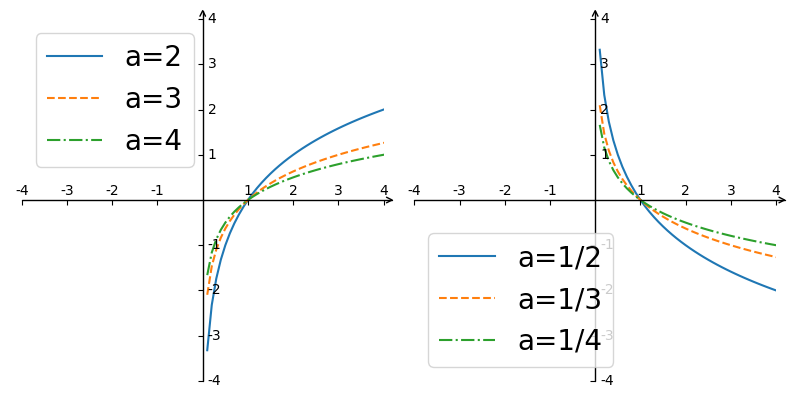
\includegraphics[height=5cm]{4.4-1.png}
\end{figure}




